\startchapter{Apply the Model on Windows C++ API}
\label{chapter:Mod}
In this section, I investigated 4 different channel types: Named pipes, MQMS, TCP/UDP socket and HTTP channels, all of which are the most fundamental ones in Windows communication framework. By matching these channels to the communication model I verified generality of the modeling. 


\section{Named Pipes Channel}
A named pipe is a named, one-way or duplex pipe for communication between the pipe server and one or more pipe clients. Both the server and client can read or write into the pipe. The pipe server and client can be on the same or different computers.  In here we only consider one server V.S one client dual-trace. One server to multiple clients scenario can always be divided into multiple server/client dual-traces. We call the end of the named pipe instance. An instance can be a server instance or a client instance. All instances of a named pipe share the same pipe name, but each instance has its own buffers and handles, and provides a separate conduit for client/server communication. 

A named pipe server responsible for the creation of the pipe, while clients of the pipe can connect to the server after it created. The creation and connection of a named pipe will return the handle ID of that pipe. As we mention before, each instance has its own handles, so the returned handle IDs of the pipe creation function of the server and pipe connection function from each client are different. These handler IDs will be used later on when messages are being sent or received to specify a pipe to which send.

\subsection{Important Channel Parameters}
There are many options for a named pipe. Some of them are critical in the perspective of the channel operations. In this sections we list the important ones.

\subsubsection{Blocking/Non-Blocking}
The named pipe channel can be opened in blocking mode or non-blocking mode. In blocking mode, when the pipe handle is specified in the ReadFile, WriteFile, or ConnectNamedPipe function, the operations are not completed until there is data to read, all data is written, or a client is connected. In non-blocking mode, ReadFile, WriteFile, and ConnectNamedPipe always return immediately. The operation fail if the channel is not ready for read, write or connection. However, since in this work we only aimed at locating the successful communication, as long as the operations success, we can locate them no matter the pipe is in blocking or non-blocking mode.

\subsubsection{Synchronous/Asynchronous}
Another critical option for named pipe channel is Synchronous/Asynchronous. In Synchronous mode, the ReadFile, WriteFile TracnsactNamedPipe and connectNamedPipe functions does not return until the operation it is performing is completed. That means we can retrieve the sent/receive message in the trace when the function return. When the channel is enable overlapped mode, the ReadFile, WriteFile TracnsactNamedPipe and connectNamedPipe functions perform asynchronously. In the asynchronous mode, ReadFile, WriteFile, TransactNamedPipe, and ConnectNamedPipe operations return immediately regardless if the operations are completed. And if the function call return ERROR\_IO\_PENDING, the calling thread then call the GetOverlappedResult function to determine the results. For the read operation, the message will be stored in the buffer indicated in the ReadFile function call when the read operation complete successfully.

\subsection{Send/Receive Scenarios}
In section \ref{modmatchresult}, I defined 13 scenarios of the general communication channel. In this section, I check their existence for named pipe channel. Some important properties of named pipe channel, which affecting the happening of the scenarios are listed in Table \ref{namedpipeproperties}. The result of the existence of the scenarios is list in Table\ref{pipematchresult} with the explanation by the affecting properties. 

\begin{table}[h]
\centering
\caption{Named Pipe Channel properties}
\label{namedpipeproperties}
\begin{tabular}{|l|p{12cm}|}
\hline
\begin{tabular}[c]{@{}l@{}}\textbf{Property} \end{tabular} & \begin{tabular}[c]{@{}l@{}}\textbf{Description}\end{tabular}\\ \hline
1 & All message going into the pipe will go out in order      \\ \hline
2 & The receiver can read multiple times to get the whole message, when he send message size is larger than the receiver's buffer  \\ \hline
3 & The receiver can only read contents from one write operation on the other end of the pipe in its one read operation                                            \\ \hline
4 & Read/Write operation return immediately when error occurs\\\hline
\end{tabular}
\end{table}

\begin{table}[h]
\centering
\caption{Send/Receive Scenarios of Named Pipe}
\label{pipematchresult}
\begin{tabular}{|l|l|l|}
\hline
\begin{tabular}[c]{@{}l@{}}\textbf{Scenario} \end{tabular} & \begin{tabular}[c]{@{}l@{}}\textbf{Existence}\end{tabular} & \begin{tabular}[c]{@{}l@{}}\textbf{Comment}\end{tabular}\\ \hline
Scenario 1 & YES & Property 1                       \\ \hline
Scenario 2 & NO  & Property 1 \\ \hline
Scenario 3 & YES & Property 4             \\ \hline
Scenario 4 & YES & Property 2 \\ \hline
Scenario 5 & NO  & Property 1                                         \\ \hline
Scenario 6 & NO  & Property 1 \\ \hline
Scenario 7 & NO  & Property 1 \\ \hline
Scenario 8 & NO  & Property 3         \\ \hline
Scenario 9 & NO  & Property 3                                                \\\hline
Scenario 10 & NO & Property 3                                               \\ \hline
Scenario 11 & NO & Property 3                                                 \\ \hline
Scenario 12 & NO & Property 3                                                 \\ \hline
Scenario 13 & NO & Property 3                                                 \\ \hline
\end{tabular}
\end{table}


\begin{figure}[h]
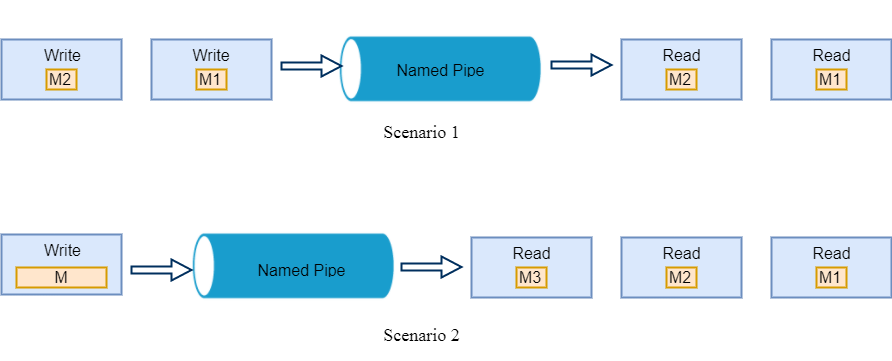
\includegraphics[scale=.48]{Figures/event}
 \caption{Two successful write/read operation scenarios. Each blue block indicate a single read or write operation.}
\label{event}
\end{figure}


\subsection{Function Calls In Each Communication Stage}
As we talk in the parameters section, Synchrounous and Asychronous mode affect the functions used to complete the send and receive operation as well as the operation of the functions. In the follow subsections, we will list the related functions for the named pipe channel for both synchronous mode and asynchronous mode. The create channel functions for both modes are the same but with different input parameters. The functions for send and receive message are also the same for both case. However, the operation of the send and receive functions are different for different mode. In addition, extra functions are being called to check the status of message sending or receiving in asynchronous mode.
\subsubsection{Synchronous}
We list all the functions that needed to locate an messaging event in a dual-trace in Table\ref{synfunctions} for synchronous named pipe. The Channel Open Functions indicate how the channel being opened/created in server and client sides, and they are different. The file name is an input parameter for CreateNamedPipe and CreateFile function. The client and server of the same pipe use the same file name. This is an important parameter to identify the pipe between the server and client in the traces. The File name is stored in the RCX register when the function is being called. The file handle is a integer return value from the CreateNamedPipe and CreateFile functions call. It will be stored in RAX register when the function return. This handle will be used as the identifier of a pipe in the client or server later on. The handle is different for server and each client even they connected to the same pipe. The send or receive message functions are the same in server and client. the file handle generated when the channel created are stored in register RCX when the WriteFile and ReadFile functions are being called. RDX holds the address of the buffer for message send or receive. The actual size of the message being sent or received are store in R9 when the function return.
  
    \begin{table}[h]
        \centering
        \caption{Functions for communication stages definition of synchronous named pipe}
        \label{synfunctions}
        \begin{tabular}{|p{1.8cm}|l|l|l|l|}
            \hline
             \multirow{2}{*}{\textbf{Stage}} &
               \multicolumn{2}{c|}{\textbf{Server}} &
               \multicolumn{2}{c|}{\textbf{Client}} \\
             \cline{2-5}
              & \textbf{Function}& \textbf{Parameters} & \textbf{Function} & \textbf{Parameters}  \\
             \hline
             \multirow{2}{*}{\parbox{1.8cm}{\textbf{Channel Open}}}
             &\multirow{2}{*}{\parbox{2.5cm}{CreateNamed- Pipe}} &  RAX: File Handler & \multirow{2}{*}{CreateFile} &  RAX: File Handler\\
              \cline{3-3} \cline{5-5}
             &&  RCX: File Name &  &  RCX: File Name\\
            \hline
             \multirow{6}{*}{\parbox{1.8cm}{\textbf{Message Send/Receive}}}
             &\multirow{3}{*}{WriteFile} &  RCX: File Handle & \multirow{3}{*}{WriteFile} &  RCX: File Handle\\
              \cline{3-3} \cline{5-5}
             &&  RDX: Buffer Address &  &  RDX: Buffer Address\\
                           \cline{3-3} \cline{5-5}
             & &  R9: Message Length &  &  R9: Message Length\\
            \cline{2-5}
             & \multirow{3}{*}{ReadFile}&  RCX: File Handle & \multirow{3}{*}{ReadFile} &  RCX: File Handle\\
              \cline{3-3} \cline{5-5}
              &&  RDX: Buffer Address &  &  RDX: Buffer Address\\
                           \cline{3-3} \cline{5-5}
             & &  R9: Message Length &  &  R9: Message Length\\
            \hline
           \multirow{2}{*}{\parbox{1.8cm}{\textbf{Channel Close}}}
             &\multirow{2}{*}{CloseHandle} & \multirow{2}{*}{RCX: File Handler} & \multirow{2}{*}{CloseHandle} &  \multirow{2}{*}{RCX: File Handler}\\
             &&   &  & \\
            \hline
        \end{tabular}
    \end{table}
\subsubsection{Asynchronous}
The functions used in Asynchronous mode for create channel, send and receive message are the same as those used in synchronous mode. However,  the ReadFile and WriteFile functions run asynchronously when the channel is asynchronous. This means the function will return immediately, even if the operation has not been completed. If the operation is complete when the function returns, the return value indicates the success or failure of the operation. Otherwise the functions return zero and GetLastError returns ERROR\_IO\_PENDING. In this case, the calling thread must wait until the operation has finished. The calling thread must then call the GetOverlappedResult function to determine the results. This means besides looking for ReadFile and WriteFile function calls in the traces, the GetOverlappedResult function should be checked in the traces to get the full result of the ReadFile or WriteFile operations. There are two scenarios of the successful communication in the dual-trace for asynchronous mode. The first one is exactly the same as synchronous situation. The second one involves the functions listed in Table\ref{asynfunctions}. In the later one, Read operation searching is bit more complicated, since ReadFile function has to be located first to get the buffer address, and then GetOverlappedResult function return should be search for the message retrieval from the memory.
    \begin{table}[h]
        \centering
        \caption{Functions for additional communication type definition of asynchronous named pipe}
        \label{asynfunctions}
        \begin{tabular}{|p{1.8cm}|l|l|l|l|}
            \hline
             \multirow{2}{*}{\textbf{Stage}} &
               \multicolumn{2}{c|}{\textbf{Server}} &
               \multicolumn{2}{c|}{\textbf{Client}} \\
             \cline{2-5}
              & \textbf{Function}& \textbf{Parameters} & \textbf{Function} & \textbf{Parameters}  \\
             \hline
             \multirow{2}{*}{\parbox{1.8cm}{\textbf{Channel Open}}}
             &\multirow{2}{*}{\parbox{2.5cm}{CreateNamed- Pipe}} &  RAX: File Handler & \multirow{2}{*}{CreateFile} &  RAX: File Handle\\
              \cline{3-3} \cline{5-5}
             &&  RCX: File Name &  &  RCX: File Name\\
            \hline
             \multirow{8}{*}{\parbox{1.8cm}{\textbf{Message Send/Receive}}}
             &\multirow{3}{*}{WriteFile} &  RCX: File Handle & \multirow{3}{*}{WriteFile} &  RCX: File Handle\\
              \cline{3-3} \cline{5-5}
             &&  RDX: Buffer Address &  &  RDX: Buffer Address\\
                           \cline{3-3} \cline{5-5}
             & &  R9: Message Length &  &  R9: Message Length\\
            \cline{2-5} 

             & \multirow{3}{*}{ReadFile}&  RAX: File Handle & \multirow{3}{*}{ReadFile} &  RCX: File Handle\\
              \cline{3-3} \cline{5-5}
              &&  RDX: Buffer Address &  &  RDX: Buffer Address\\
                           \cline{3-3} \cline{5-5}
             & &  R9: Message Length &  &  R9: Message Length\\
              \cline{2-5} 
             & \multirow{2}{*}{\parbox{2.5cm}{GetOver- lappedResult}}&  RCX: File Handler & \multirow{2}{*}{\parbox{2.5cm}{GetOver- lappedResult}} &  RCX: File Handler\\
              \cline{3-3} \cline{5-5}
             & &  RDX:  OVERLAPPED&  &  RDX:  OVERLAPPED\\
                         \hline
                         
                          \multirow{2}{*}{\parbox{1.8cm}{\textbf{Channel Close}}}
             &\multirow{2}{*}{CloseHandle} & \multirow{2}{*}{RCX: File Handler} & \multirow{2}{*}{CloseHandle} &  \multirow{2}{*}{RCX: File Handler}\\
             &&   &  & \\
            \hline
        \end{tabular}
    \end{table}
    


\section{MQMS Channel}
Message Queuing (MSMQ) is designed for communication between applications which is running at different times across heterogeneous networks and systems that may be temporarily offline. Messages are sent to and read from queues by applications. Multiple sending applications can send messages to and multiple receiving applications can read messages from one queue. \cite{redkar2004pro}

However, in this work only one sending application versus one receiving application case is considered. Multiple sender to multiple receiver scenario can always be divided into multiple sender/receiver dual-traces. 

The sending or receiving application can create the queue or use the existing one. However, both of them have to open the queue before they access it. The handle ID returned by the open queue function will be used later on when messages are being sent or received

\subsection{Important Channel Parameters}    
Same as Named pipe channels, MSMQ channel have many options or settings affecting the operations happen in the channels. In this section I listed those ones affecting the dual trace analysis. 

\subsubsection{Synchronous/Asynchronous Receiving}
In Message Queuing channels, only receiving can operate in asynchronous mode. When synchronously reading messages, the input parameters fnReceiveCallback and lpOverlapped are set to NULL. The calling thread is blocked until a suitable message is available or a time-out occurs for the receiving function. When asynchronously reading messages, MQReceiveMessage returns MQ\_OK if a suitable message is found. Otherwise, MQReceiveMessage returns immediately with the return value MQ\_INFORMATION\_OPERATION\_PENDING. This return value indicates that the operation is pending and will be completed as soon as a suitable message can be found. Further operations needed to get the message later on. More details about the further operations will be described in Section \ref{callback}
\subsubsection{Asynchronous Receiving With Call Back Functio or Completion port}\label{callback}
When the receiving operates in asynchronous mode, completion ports or call back function can be used for the asynchronously reading. 

In the completion port using situation, MQGetOverlappedResult is called to retrieve the success or error code from the OVERLAPPED structure. If no message is received before the time-out period elapses, an error is returned, and the start routine returns, terminating the thread in an implicit call to ExitThread.

In the call back function using situation, a call back function's pointer is given when the receiving function is being called. The call back function will perform its task as long a message was received or the time-out interval supplied by the caller elapsed.
\subsubsection{Message Properties Description Structure}

\subsection{Send/Receive Scenarios}
In this section, I check the scenarios existence for message queuing. Some important properties of MSMQ channel, which affecting the happening of the scenarios are listed in Table \ref{msmqproperties}. The result of the existence of the scenarios is list in Table\ref{msmqmatchresult} with the explanation by the affecting properties. 

\begin{table}[h]
\centering
\caption{Named Pipe Channel properties}
\label{msmqproperties}
\begin{tabular}{|l|p{12cm}|}
\hline
\begin{tabular}[c]{@{}l@{}}\textbf{Property} \end{tabular} & \begin{tabular}[c]{@{}l@{}}\textbf{Description}\end{tabular}\\ \hline
1 & All message going into the pipe will go out in order      \\ \hline
2 & The receiver can read multiple times to get the whole message, when he send message size is larger than the receiver's buffer  \\ \hline
3 & The receiver can only read contents from one write operation on the other end of the pipe in its one read operation                                            \\ \hline
4 & Read/Write operation return immediately when error occurs\\\hline
\end{tabular}
\end{table}

\begin{table}[h]
\centering
\caption{Send/Receive Scenarios of Named Pipe}
\label{msmqmatchresult}
\begin{tabular}{|l|l|l|}
\hline
\begin{tabular}[c]{@{}l@{}}\textbf{Scenario} \end{tabular} & \begin{tabular}[c]{@{}l@{}}\textbf{Existence}\end{tabular} & \begin{tabular}[c]{@{}l@{}}\textbf{Comment}\end{tabular}\\ \hline
Scenario 1 & YES & Property 1                       \\ \hline
Scenario 2 & NO  & Property 1 \\ \hline
Scenario 3 & YES & Property 4             \\ \hline
Scenario 4 & YES & Property 2 \\ \hline
Scenario 5 & NO  & Property 1                                         \\ \hline
Scenario 6 & NO  & Property 1 \\ \hline
Scenario 7 & NO  & Property 1 \\ \hline
Scenario 8 & NO  & Property 3         \\ \hline
Scenario 9 & NO  & Property 3                                                \\\hline
Scenario 10 & NO & Property 3                                               \\ \hline
Scenario 11 & NO & Property 3                                                 \\ \hline
Scenario 12 & NO & Property 3                                                 \\ \hline
Scenario 13 & NO & Property 3                                                 \\ \hline
\end{tabular}
\end{table}



\subsection{Function Calls In Each Communication Stage}
We list all the functions that needed to locate an messaging event in a dual-trace in Table\ref{synfunctions} for MSMQ. The Channel Open Functions indicate how the channel being opened in sending and receiving sides. The Queue Format Name is an input parameter for MQOpenQueue function. This is an important parameter to identify the queue. The File name is stored in the RCX register when the function is being called. The queue handle is a integer return value from the MQOpenQueue functions call. It will be stored in RAX register when the function return. The handle is different for each application using the same queue. The queue handle generated when the queue is opened by an application are stored in register RCX when the MQSendMessage or MQReceiveMessage functions are being called for message sending and receiving. RDX holds the address of the sending message structure for message sending while R9 holds the address of the receiving message structure for message receiving. For message receiving, the operation can be synchronous or asynchronous. For the asynchronous receiving, an callback function's pointer is indicated in the parameter fnReceiveCallback which is pushed on the stack if the callback function is employed. If the call back function is not employed, MQGetOverlappedResult should be called to get the received message.

\subsubsection{Synchronous Receiving}
The functions used for defining a communication channel and events are listed in Table\ref{msmqsynfunctions}.
    \begin{table}[h]
        \centering
        \caption{Functions for communication stages of MSMQ for synchronous receiving}
        \label{msmqsynfunctions}
        \begin{tabular}{|l|l|l|}
            \hline
             \textbf{Stage} & \textbf{Function}& \textbf{Parameters}  \\
             \hline
             \multirow{2}{*}{{\textbf{Channel Open}}}
             &\multirow{2}{*}{{MQOpenQueue}} &  RAX: Queue Handler\\
              \cline{3-3} 
             & &  RCX: Queue Format Name\\
            \hline
             \multirow{4}{*}{{\textbf{Message Send/Receive}}}
             &\multirow{2}{*}{MQSendMessage} &  RCX: Queue Handle \\
              \cline{3-3} 
             &&  RDX: Message description structure Address \\
            \cline{2-3}
             & \multirow{2}{*}{MQReceiveMessage}&  RCX: Queue Handle \\
              \cline{3-3} 
              &&  R9: Message description structure Address \\
            \hline
            \textbf{Channel Close} &MQCloseQueue & RCX: Queue Handler \\
            \hline
        \end{tabular}
    \end{table}

\subsubsection{Asynchronous Receiving with Call Back Functions}
The functions used for defining a communication channel and events are listed in Table\ref{msmqasynfunctionscallback}.
    \begin{table}[h]
        \centering
        \caption{Functions for communication stages of MSMQ for asynchronous receiving with call back function}
        \label{msmqasynfunctionscallback}
        \begin{tabular}{|l|l|l|}
            \hline
             \textbf{Stage} & \textbf{Function}& \textbf{Parameters}  \\
             \hline
             \multirow{2}{*}{{\textbf{Channel Open}}}
             &\multirow{2}{*}{{MQOpenQueue}} &  RAX: Queue Handler\\
              \cline{3-3} 
             & &  RCX: Queue Format Name\\
            \hline
             \multirow{5}{*}{\parbox{2.5cm}{\textbf{Message Send/Receive}}}
             &\multirow{2}{*}{MQSendMessage} &  RCX: Queue Handle \\
              \cline{3-3} 
             &&  RDX: Message description structure Address \\
            \cline{2-3}
             & \multirow{3}{*}{\parbox{2.5cm}{MQReceive-Message}}&  RCX: Queue Handle \\
              \cline{3-3} 
              &&  R9: Message description structure Address \\
                            \cline{3-3} 
              &&  Stack(The Third One): Pointer of the call back function \\
            \hline
            \textbf{Channel Close} &MQCloseQueue & RCX: Queue Handler \\
            \hline
        \end{tabular}
    \end{table}


\subsubsection{Asynchronous Receiving without Call Back Functions}
The functions used for defining a communication channel and events are listed in Table\ref{msmqasynfunctions}.
    \begin{table}[h]
        \centering
        \caption{Functions for communication stages of MSMQ for asynchronous receiving without call back function}
        \label{msmqasynfunctions}
        \begin{tabular}{|l|l|l|}
            \hline
             \textbf{Stage} & \textbf{Function}& \textbf{Parameters}  \\
             \hline
             \multirow{2}{*}{{\textbf{Channel Open}}}
             &\multirow{2}{*}{{MQOpenQueue}} &  RAX: Queue Handler\\
              \cline{3-3} 
             & &  RCX: Queue Format Name\\
            \hline
             \multirow{5}{*}{\parbox{2.5cm}{\textbf{Message Send/Receive}}}
             &\multirow{2}{*}{MQSendMessage} &  RCX: Queue Handle \\
              \cline{3-3} 
             &&  RDX: Message description structure Address \\
            \cline{2-3}
             & \multirow{3}{*}{\parbox{2.5cm}{MQReceive-Message}}&  RCX: Queue Handle \\
              \cline{3-3} 
              &&  R9: Message description structure Address \\
                            \cline{3-3} 
              &&  Stack(The Fourth One): Overlap Structure address\\
                          \cline{2-3}
                          
              & \multirow{2}{*}{\parbox{2.5cm}{MQGetOver-lappedResult}} &  RCX: Overlap Structure address  \\
              &&\\
            \hline
            \textbf{Channel Close} &MQCloseQueue & RCX: Queue Handler \\
            \hline
        \end{tabular}
    \end{table}
\section{TCP/UDP Socket Channel}


<<<<<<< HEAD
\section{Verification}
\subsection{Executable Disassemble}

=======
>>>>>>> dbf06a633ced520911200a79b9a179fb20e14b6f

